% This is text associated with the open textbook "Open Electromagnetics"
% See immediately below for author, date
% This work is licensed under the Creative Commons Attribution-ShareAlike 4.0 International License. (CC BY-SA 4.0) 
% To view a copy of the license, visit http://creativecommons.org/licenses/by-sa/4.0/

%ORB TITLE Parallel Plate Waveguide: The TM$_0$ Mode
%ORB AUTHOR 0        # S.W. Ellingson, Virginia Tech (ellingson@vt.edu)
%ORB DATE 20191202   # yyyymmdd
%ORB ABSTRACT 

\label{m0220_Parallel_Plate_Waveguide_TM0_Mode} % <-- Must match name of this file and module directory name.  Don't mess with this!
\index{waveguide!parallel plate|(}
\index{parallel-plate waveguide|see{waveguide}}

In Section~\ref{m0173_Parallel_Plate_Waveguide_Introduction}, the parallel plate waveguide (also shown in Figure~\ref{m0220_fParallelPlateWaveguide}) was introduced.
%
\begin{figure}[b!] % <--- "[b]" for first figure in section *only*; delete for 2nd and subsequent figures
\begin{center}
\pdftooltip{{  % note double braces
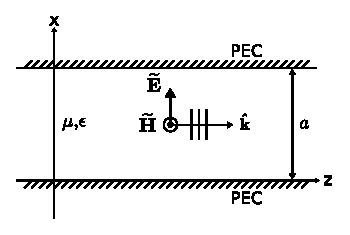
\includegraphics[width=0.8\columnwidth]{modules/m0220_fParallelPlateWaveguide.eps} 
% https://commons.wikimedia.org/wiki/File:TM_component_of_electric_field_in_parallel_plate_waveguide.svg
}}{In a z-x Cartesian coordinate system, two parallel plates separated a distance small a. Interior region small mu comma small epsilon. Electric field in positive x direction and magnetic field intensity out of page. A plane wave moves in the positive z direction.}
\end{center}
\centerline{\scriptsize 
\copyright~\hyperref[m0220_fParallelPlateWaveguide_Credit]{C.\ Wang} 
\href{https://creativecommons.org/licenses/by-sa/4.0/}{CC BY-SA 4.0} 
(modified)
} % \centerline 
\caption{
\label{m0220_fParallelPlateWaveguide}
TM$_0$ mode in a parallel plate waveguide.
}
\end{figure}
%
At the end of that section we decomposed the problem into its constituent TE and TM fields.
In Section~\ref{m0177_Parallel_Plate_Waveguide_TM_Electric}, we determined the electric field component of the TM field, which was found to consist of a set of discrete modes.
In this section, we address the lowest-order ($m=0$) mode of the TM field, which has special relevance in a number of applications including microstrip transmission lines.
This mode is commonly referred to as the ``TM$_0$'' mode.

The TM electric field intensity in the waveguide is given by Equation~\ref{m0177_eEsum} with modal components determined as indicated by Equations~\ref{m0177_efcm}--\ref{m0177_ekxma} (Section~\ref{m0177_Parallel_Plate_Waveguide_TM_Electric}).
Recall that the $m=0$ mode can only exist only in the TM case, and does not exist in the TE case.
We also noted that the cutoff frequency for this mode is zero, so it may exist at any frequency, and within any non-zero plate separation $a$.
For this mode $k_x^{(0)} = 0$, $k_z^{(0)}=\beta$, and we find
%
\begin{equation}
\widetilde{\bf E} = \hat{\bf x} E_{x0}^{(0)} e^{-j\beta z}  ~~~ \mbox{(TM$_0$ mode)}
\end{equation}
%
Remarkably, we find that this mode has the form of a uniform plane wave which propagates in the $+\hat{\bf z}$ direction; i.e., squarely between the plates.
The phase and group velocities of this wave are equal to each other and $\omega/\beta$, precisely as expected for a uniform plane wave in unbounded media; i.e., as if the plates did not exist.
This observation allows us to easily determine the associated \emph{magnetic} field:
Using the plane wave relationship,
\index{plane wave relationships}
%
\begin{flalign}
\widetilde{\bf H} &= \frac{1}{\eta}\hat{\bf k} \times \widetilde{\bf E} \\
                  &= \frac{1}{\eta}\hat{\bf z} \times \left( \hat{\bf x} E_{x0}^{(0)} e^{-j\beta z} \right) \\
                  &= \hat{\bf y} \frac{E_{x0}^{(0)}}{\eta} e^{-j\beta z}  ~~~ \mbox{(TM$_0$ mode)}
\end{flalign}

%%%%%%%%%%%%%%%%%%%%%%%%%%%%%%%%%%%%%%%%%%%%%%%
%ORB EXAMPLE
~\\ \begin{example} 
\begin{mdframed}[backgroundcolor=brown!20,linecolor=brown!20]\raggedright
Guided waves in a printed circuit board (PCB).
\\~\\
A very common form of PCB consists of a 1.575~mm-thick slab of low-loss dielectric having relative permittivity $\approx 4.5$ sandwiched between two copper planes.
Characterize the electromagnetic field in a long strip of this material.
Assume a single source exists at one end of the strip, and operates at frequencies below 10~GHz.

{\bf Solution.}
Let us assume that the copper planes exhibit conductivity that is sufficiently high that the inward-facing surfaces may be viewed as perfectly-conducting.
Also, let us limit scope to the field deep within the ``sandwich,'' and neglect the region near the edges of the PCB.
Under these conditions, the PCB is well-modeled as a parallel-plate waveguide.
Thus, the electromagnetic field consists of a combination of TE and TM modes.
The active (non-zero) modes depend on the source (a mode must be ``stimulated'' by the source in order to propagate) and modal cutoff frequencies.
The cutoff frequency for mode $m$ is 
%
\begin{equation}
f^{(m)}_c = \frac{m}{2a\sqrt{\mu\epsilon}}
\end{equation}
%
In this case, $a=1.575$~mm, $\mu\approx\mu_0$, and $\epsilon\approx 4.5\epsilon_0$.  Therefore:
%
\begin{equation}
f^{(m)}_c \approx \left( 44.9~\mbox{GHz} \right) m
\end{equation}
%
Since the cutoff frequency for $m=1$ is much greater than 10~GHz, we may rest assured that the only mode that can propagate inside the PCB is TM$_0$.
Therefore, the field deep inside the PCB may be interpreted as a single plane wave having the TM$_0$ structure shown in Figure~\ref{m0220_fParallelPlateWaveguide}, propagating away from the source end of the PCB.
The phase velocity is simply that of the apparent plane wave:
%
\begin{equation}
v_p = \frac{1}{\sqrt{\mu\epsilon}} \approx 1.41 \times 10^8~\mbox{m/s} \approx 0.47c
\end{equation}
%
\end{mdframed}
% note figures will need to go between "\end{mdframed}" and "\end{example}"
\end{example}
%%%%%%%%%%%%%%%%%%%%%%%%%%%%%%%%%%%%%%%%%%%%%%%
%
The scenario described in this example is essentially a very rudimentary form of microstrip transmission line.
\index{microstrip}

\index{waveguide!parallel plate|)}

